In the scope of simplifying the configuration of a given product line some specific tools and techniques were used. This section will give an overview of what was used in this work to archive the simplification.

\subsection{Feature Models}
Feature models are multi-purpose tool for product lines. Figure~\ref{img-fm} shows a simplified example of a feature model.
\begin{figure}
	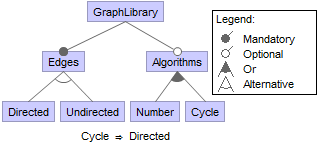
\includegraphics{img/img-fm.png}
	\caption{A simple example of a feature model}
	\label{img-fm}
\end{figure}
Amongst their benefits are:
\begin{itemize}
\item Visualization of the possible features and their hierarchy
\item Classification of features and their dependencies (alternative/or; optional/mandatory/abstract)
\item Formal Representation of the whole product line $\Rightarrow$ computationally processable
\item Assistance/foundation for configuration and variant validation
\end{itemize}
They are basically structured like trees: There is a root node, an arbitrary number of levels of nodes and finally leaf nodes without child nodes of their own. In that manner feature models map the hierarchy of features. In addition they mark each feature as either mandatory or optional as well as either abstract or concrete. The possible relationships of multiple features with a mutual parent feature are \textit{OR} (at least one feature has to be selected), \textit{ALTERNATIVE} (exactly one feature has to be selected) and \textit{AND} (any number of features can be selected). As features' relations may be of higher complexity than just parent-child relations additional constraints can be noted within a feature model. Constraints are boolean expressions, the example in figure~\ref{img-fm} shows an implication.

\subsection{Product configuration}
Through configuration a concrete product can be derived from a product line. Each valid configuration represents a specific \textit{variant} of the possible products.

During configuration a user selects or unselects features to his needs. This process requires a lot of domain knowledge on the one hand and detailed information about each single feature on the other. With growing numbers of possible features (and thus growing numbers of possible variants) configuration get more and more complex and turns out to be not trivial.

One of the purposes of the feature-oriented approach is saving the effort of creating a whole new product and deriving that product from a product line instead. The sheer overhead of configuration might even negate that benefit if configuration grows too complex.

\subsection{Constraints, contradictions, SAT-solver}
As stated above a feature model may contain constraints in the form of boolean expressions. Also, the feature-tree can be expressed as a boolean statement. The model shown in figure~\ref{img-fm} can be expressed as follows:
\begin{equation}
\begin{split}
	GraphLibrary\ \wedge\ Edges\\
	\wedge\ ((Directed\ \wedge \neg Undirected)\\
	\vee (\neg Directed\ \wedge\ Undirected))\\
	\wedge\ (Algorithms\ \Rightarrow\ (Number\ \vee\ Cycle))\\
	\wedge\ (Cycle\ \Rightarrow\ Directed)
\end{split}
\end{equation}\\
This formalism allows a configuration to be checked for validity. To do so each selected Feature is appended with a logical \textit{AND} and each specifically unselected feature is also appended with a logical \textit{AND} but gets negated. The resulting expression is then evaluated by a SAT-solver to check for satisfiability. Even during configuration this process can be applied to check for invalid partial configurations after each decision.
